\chapter{Thiết kế kiến trúc hệ thống}
\label{chp:04}

\section{Tổng quan kiến trúc Platform}

Để đảm bảo tính linh hoạt, khả năng mở rộng và tái sử dụng, hệ thống được thiết kế dựa trên mô hình phân lớp chức năng. Kiến trúc này cho phép tách biệt giữa hạ tầng phần cứng vật lý và logic thực thi của ứng dụng AI.

\begin{figure}[!h]
\centering
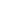
\includegraphics[width=0.6\textwidth]{chapter04/img/platform.png}
\caption{Stack kiến trúc hệ thống Edge-AI}
\end{figure}

\begin{itemize}
    \item Lớp 1: Hardware Layer (Cơ sở hạ tầng)Phân tích lý do chọn Zynq 
    làm Host (Quản lý I/O tốt, chạy Linux) và CV32E40P làm Accelerator 
    (Lõi nhỏ gọn, hỗ trợ tập lệnh IMC, tối ưu diện tích chip)
    .Nhấn mạnh vào khối AXI Interconnect và BRAM Controller 
    (Phiên dịch viên ngôn ngữ bus) - Đây chính là xương sống của Platform.
    \item Lớp 2: Software / Runtime Layer (Hệ điều hành \& Trình điều khiển)
    Trình bày luồng hoạt động (Data Flow): ARM đóng vai trò Master, 
    dùng Memory Mapped I/O để đẩy dữ liệu. RISC-V đóng vai trò Slave, 
    luôn ở trạng thái chờ lệnh (Polling)
    ARM chụp ảnh $\rightarrow$
    Đẩy vào BRAM $\rightarrow$ Kích hoạt cờ (Flag) $\rightarrow$ 
    RISC-V đọc cờ $\rightarrow$ Tính toán $\rightarrow$ Ghi kết quả 
    $\rightarrow$ ARM đọc kết quả.
    \item Lớp 3: Application Layer (Tầng ứng dụng): Một 
    nền tảng "mở". Hiện tại đang chạy nhận diện người (CNN), nhưng vì 
    là Platform, ngày mai người dùng hoàn toàn có thể nạp firmware 
    khác để chạy nhận diện âm thanh mà không cần sửa lại phần cứng.
\end{itemize}


\subsection{Layer 1: Hardware Layer}
Đây là tầng thấp nhất của nền tảng, thực thi các tác vụ tính toán cường độ cao và quản lý luồng dữ liệu thô. Thành phần chính bao gồm:

Hệ thống xử lý (Processing System - PS): Tận dụng cụm lõi ARM Cortex-A53 của Zynq UltraScale+ để điều phối toàn hệ thống.

Bộ gia tốc lõi mềm (Soft-core Accelerator): Lõi vi xử lý RISC-V CV32E40P kết hợp cùng khối tăng tốc phần cứng (CNN Accelerator) tùy chỉnh trên vùng Programmable Logic (PL).

Hệ thống di chuyển dữ liệu (Data Mover): Tích hợp khối DMA Controller và mạng lưới AXI4 Interconnect để vận chuyển dữ liệu giữa DDR4 và Shared BRAM với độ trễ thấp nhất, giảm thiểu gánh nặng cho CPU trung tâm.

\subsection{layer 2: software / runtime layer}
Đóng vai trò là "cầu nối" (Middleware) giúp lớp ứng dụng có thể tương tác với phần cứng một cách minh bạch:

Host Environment: Hệ điều hành Linux chạy trên lõi ARM, cung cấp các Driver giao tiếp Camera, bộ nhớ và thư viện tiền xử lý ảnh (OpenCV).

Communication Protocol: Hiện thực hóa cơ chế Memory-Mapped I/O và giao thức bắt tay thông qua các cờ hiệu (Flags) trong bộ nhớ dùng chung.

Firmware Subsystem: Chứa mã nguồn Bare-metal tối ưu hóa cho RISC-V, bao gồm các thư viện toán tử AI cơ bản và trình điều khiển khối tăng tốc phần cứng.

\subsection{layer 3: application layer}
Đây là tầng cao nhất, quy định kịch bản sử dụng thực tế của hệ thống. 
\begin{itemize}
    \item \textbf{Ứng dụng kiểm chứng (Use-case):} Hiện tại, tầng này đang thực thi cấu trúc mạng \textbf{MobileNetV2} (lượng tử hóa INT8) để giải quyết bài toán phát hiện người (Human Detection) trên tập dữ liệu INRIA.
    \item \textbf{Tính linh hoạt trong cùng miền ứng dụng (Domain-Specific Flexibility):} Nhờ thiết kế phân lớp, người dùng có thể dễ dàng chuyển đổi hệ thống sang giải quyết bài toán khác trong cùng lĩnh vực thị giác máy tính (ví dụ: chuyển từ MobileNet sang nhận diện biển báo giao thông bằng kiến trúc CNN khác). Việc này chỉ yêu cầu cập nhật tệp trọng số và mã nguồn Firmware (C/C++) ở Layer 2, mà hoàn toàn không cần can thiệp hay tổng hợp lại kiến trúc vật lý ở Layer 1.
\end{itemize}

\section{kiến trúc dị thể}
Hệ thống Edge-AI được thiết kế dựa trên kiến trúc không đồng nhất 
(Heterogeneous Architecture) của nền tảng Zynq UltraScale+ MPSoC trên bo mạch Kria KV260. 
Thiết kế tận dụng mô hình đồng thiết kế phần cứng/phần mềm (Hardware/Software Co-design)
 để tối ưu hóa hiệu năng xử lý.

\begin{figure}[!h]
\centering
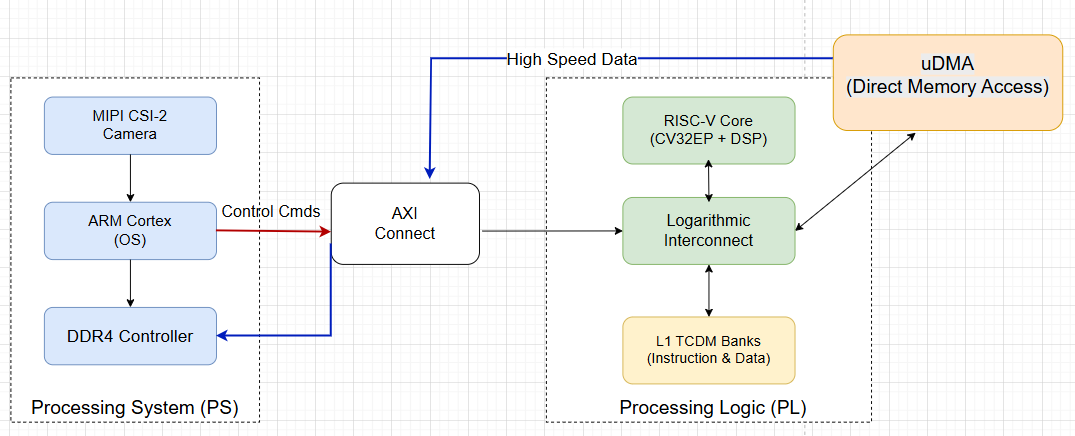
\includegraphics[width=1\textwidth]{chapter04/img/arch.png}
\caption{Kiến trúc hệ thống tổng quan}
\label{fig:proposed_architecture}
\end{figure}

Mô hình tổng thể được chia thành hai miền xử lý chính:
\begin{itemize}
    \item Processing System
    \item Khối Cầu nối
    \item Programmable Logic
\end{itemize}

Như thể hiện tại Hình \ref{fig:proposed_architecture}, hệ thống được phân chia thành ba miền xử lý chính với các vai trò chuyên biệt:

\begin{itemize}
    \item \textbf{Phân hệ Xử lý (Processing System - PS):} 
    Đóng vai trò là khối điều khiển trung tâm (Host), hoạt động trên nền tảng vi xử lý ARM Cortex-A53 lõi tứ. PS chịu trách nhiệm:
    \begin{itemize}
        \item Quản lý tài nguyên hệ thống và khởi chạy quy trình boot.
        \item Giao tiếp với các ngoại vi tiêu chuẩn như Camera (qua giao diện MIPI CSI-2) và Màn hình.
        \item Thực hiện các bước tiền xử lý hình ảnh (Preprocessing) và quản lý bộ nhớ đệm dữ liệu (Data Buffering) trên DDR4.
    \end{itemize}

    \item \textbf{Khối Giao tiếp Liên kết (Interconnect Fabric):} 
    Đóng vai trò là cầu nối dữ liệu tốc độ cao, sử dụng giao thức chuẩn công nghiệp AMBA AXI4. Khối này bao gồm các bộ chuyển mạch thông minh (AXI SmartConnect) để:
    \begin{itemize}
        \item Phân tách luồng điều khiển (Control Plane) băng thông thấp và luồng dữ liệu (Data Plane) băng thông cao.
        \item Đảm bảo đồng bộ hóa giữa hai miền xung nhịp khác nhau của PS và PL.
        \item Cho phép truy cập bộ nhớ chia sẻ (Shared Memory) một cách trong suốt giữa các vi xử lý.
    \end{itemize}

    \item \textbf{Phân hệ Logic Khả trình (Programmable Logic - PL):} 
    Đóng vai trò là bộ tăng tốc tính toán (Accelerator). Tại đây, tài nguyên FPGA được cấu hình để triển khai một Hệ thống trên Chip (SoC) con, bao gồm:
    \begin{itemize}
        \item \textbf{Lõi vi xử lý mềm RISC-V (PULP Subsystem):} Điều phối luồng thực thi thuật toán AI.
        \item \textbf{Bộ tăng tốc phần cứng (CNN Accelerator):} Thực hiện các phép toán tích chập chuyên sâu.
        \item \textbf{Cơ chế truy cập bộ nhớ trực tiếp (uDMA):} Tối ưu hóa việc di chuyển dữ liệu ảnh mà không làm gián đoạn CPU.
    \end{itemize}
\end{itemize}

Sự kết hợp chặt chẽ giữa ba thành phần này cho phép hệ thống hoạt động theo cơ chế đường ống (Pipelining), đảm bảo khả năng xử lý hình ảnh thời gian thực với độ trễ thấp nhất.

%=======================================================================
\newpage
\section{Thiết kế Processing System}

Đây là phần cứng có sẵn (Hard-core) trên chip Zynq UltraScale+ của board Kria KV260.
\begin{itemize}
    \item ARM Cortex-A53: Đóng vai trò là CPU chủ (Host). Nó có thểchạy hệ điều hành (Linux hoặc Bare-metal) 
để quản lý toàn bộ hệ thống. Nhiệm vụ của nó là giao tiếp với Camera (qua cổng MIPI), 
nhận ảnh, tiền xử lý (resize, crop) và lưu trữ ảnh vào bộ nhớ lớn.
    \item DDR4 Controller (Shared Memory): Đây là kho chứa dữ liệu chung. Vì bộ nhớ trong của RISC-V 
rất nhỏ (chỉ vài chục KB), toàn bộ dữ liệu ảnh đầu vào (Image Buffer) phải được lưu ở đây 
(4GB RAM của Kria).
\end{itemize}

PS đóng vai trò "Master" điều phối, gửi lệnh "Bắt đầu" (Start) cho khối PL 
khi đã có dữ liệu ảnh sẵn sàng.

\subsection{Cấu hình chi tiết các phân hệ}

\subsubsection{Khối xử lý ứng dụng (APU Configuration)}
Trung tâm của PS là cụm vi xử lý Quad-core ARM Cortex-A53 hoạt động ở tần số 1.2 GHz. Trong thiết kế này, APU được cấu hình để:
\begin{itemize}
    \item \textbf{Chế độ hoạt động:} Chạy hệ điều hành PetaLinux (dựa trên Yocto Project) để tận dụng các driver có sẵn cho Camera MIPI và ngăn xếp mạng (Network Stack).
    \item \textbf{Quản lý Boot:} Sử dụng giao diện SD Card (SD1) kết nối với các chân MIO để nạp bitstream cho FPGA và khởi động hệ thống.
\end{itemize}

\subsubsection{Cấu hình Giao diện Bộ nhớ (DDR Configuration)}
Bộ điều khiển DDR4 (DDRC) được kích hoạt để quản lý 4GB RAM tích hợp trên Kria SOM. Cấu hình này rất quan trọng vì nó đóng vai trò là "Shared Memory" cho cả hệ thống:
\begin{itemize}
    \item \textbf{Data Width:} 64-bit (hỗ trợ băng thông cao).
    \item \textbf{AXI Port QoS:} Cổng S\_AXI\_HP0 được ưu tiên mức Quality of Service (QoS) cao để đảm bảo uDMA không bị nghẽn khi ghi dữ liệu ảnh, tránh hiện tượng rớt khung hình (frame drop).
\end{itemize}

\subsubsection{Cấu hình Giao diện PS-PL (Interface Configuration)}
Để kết nối với miền Logic khả trình (nơi chứa RISC-V và Accelerator), hai cổng giao tiếp AXI quan trọng được kích hoạt:

\begin{enumerate}
    \item \textbf{M\_AXI\_HPM0\_FPD (Master):}
    \begin{itemize}
        \item \textit{Chức năng:} Cổng Master hiệu năng cao miền công suất thấp (Full Power Domain).
        \item \textit{Nhiệm vụ:} Dùng để CPU ARM gửi tín hiệu điều khiển, cấu hình thanh ghi và nạp firmware vào bộ nhớ lệnh của RISC-V.
        \item \textit{Độ rộng:} 32-bit (phù hợp với bus AXI-Lite).
    \end{itemize}
    
    \item \textbf{S\_AXI\_HP0\_FPD (Slave):}
    \begin{itemize}
        \item \textit{Chức năng:} Cổng Slave hiệu năng cao (High Performance).
        \item \textit{Nhiệm vụ:} Cho phép các Master bên phía FPGA (cụ thể là uDMA) truy cập trực tiếp vào RAM DDR4.
        \item \textit{Độ rộng:} 128-bit (để tối đa hóa tốc độ truyền tải ảnh).
    \end{itemize}
\end{enumerate}

\subsubsection{Cấu hình Xung nhịp (Clock Configuration)}
Khối PS cung cấp nguồn xung nhịp tham chiếu cho toàn bộ logic bên phía PL 
thông qua chân \texttt{pl\_clk0}. Tần số được thiết lập là \textbf{100 MHz}, 
đảm bảo sự cân bằng giữa tốc độ xử lý của nhân RISC-V và mức tiêu thụ năng lượng.

%=========================================================
\newpage
\section{Thiết kế Hệ thống Giao tiếp và Bộ nhớ (Interconnect \& Memory Hierarchy)}
\label{sec:interconnect_design}

Trong kiến trúc SoC dị thể, hiệu năng của hệ thống không chỉ phụ thuộc vào tốc độ xử lý của từng nhân (Core) mà còn phụ thuộc vào băng thông và độ trễ của hệ thống kết nối. Mục này trình bày thiết kế chi tiết mạng lưới giao tiếp giữa PS và PL, cùng với quy hoạch không gian bộ nhớ chung.

\begin{figure}[h]
    \centering
    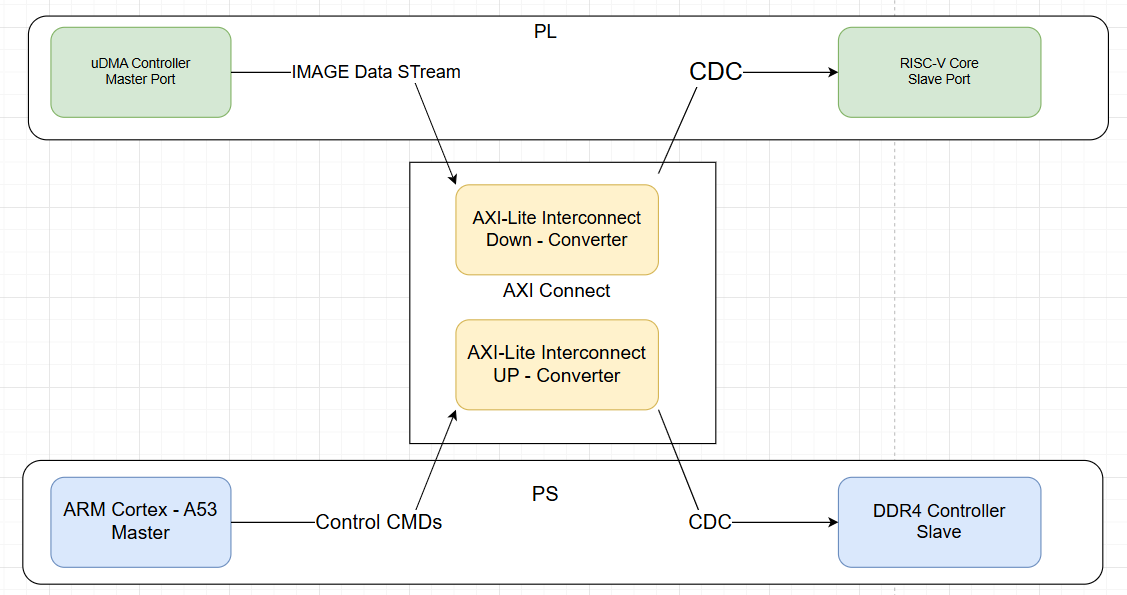
\includegraphics[width=1\textwidth]{chapter04/img/axi_arch.png}  
    \caption{Sơ đồ khối hệ thống giao tiếp AXI giữa PS và PL.}
    \label{fig:axi_interconnect}
\end{figure}


\subsection{Cơ chế AXI SmartConnect (PS-PL Bridge)}
Để kết nối miền xử lý ứng dụng (PS) hoạt động ở tần số cao và miền logic khả trình (PL) hoạt động ở tần số thấp, hệ thống sử dụng khối IP **AXI SmartConnect**. Đây không chỉ là dây dẫn đơn thuần mà là một ma trận chuyển mạch thông minh (Switch Fabric) đảm nhiệm ba chức năng:
\begin{itemize}
    \item \textbf{Clock Domain Crossing (CDC):} Đồng bộ hóa tín hiệu giữa miền xung nhịp PS (1.2 GHz) và miền PL (100 MHz) bằng các bộ đệm FIFO bất đồng bộ, đảm bảo không xảy ra lỗi Metastability.
    \item \textbf{Width Conversion:} Chuyển đổi độ rộng dữ liệu tự động giữa bus hệ thống 128-bit (phía DDR) và bus ngoại vi 32-bit (phía RISC-V).
    \item \textbf{Arbitration:} Phân giải tranh chấp khi nhiều Master cùng truy cập bộ nhớ.
\end{itemize}

Hệ thống được thiết kế với hai kênh giao tiếp vật lý tách biệt:

\subsubsection{Kênh Điều khiển (Control Path - AXI4-Lite)}
Đây là tuyến giao tiếp từ \textbf{Master (ARM Cortex-A53)} đến \textbf{Slave (PULP Subsystem)}.
\begin{itemize}
    \item \textbf{Giao thức:} AXI4-Lite 32-bit. Đây là phiên bản rút gọn của AXI4, không hỗ trợ truyền tải dạng Burst.
    \item \textbf{Mục đích:} Tối ưu hóa cho các giao dịch đơn lẻ, độ trễ thấp.
    \item \textbf{Chức năng:} Dùng để CPU ARM thực hiện các tác vụ quản trị như:
    \begin{itemize}
        \item Cấu hình thanh ghi điều khiển của bộ tăng tốc CNN (Trọng số, Bias, Kích thước ảnh).
        \item Gửi tín hiệu kích hoạt (Trigger) quá trình suy luận.
        \item Reset mềm (Soft-reset) khối PL trong trường hợp treo hệ thống.
    \end{itemize}
\end{itemize}

\subsubsection{Kênh Dữ liệu (Data Path - AXI4-Full)}
Đây là tuyến giao tiếp từ \textbf{Master (uDMA Controller)} đến \textbf{Slave (DDR4 Controller)}.
\begin{itemize}
    \item \textbf{Giao thức:} AXI4-Full 128-bit.
    \item \textbf{Mục đích:} Tối ưu hóa băng thông (Throughput).
    \item \textbf{Chức năng:} Hỗ trợ cơ chế \textit{Burst Transaction}, cho phép uDMA đọc/ghi liên tiếp tới 256 gói dữ liệu chỉ với một địa chỉ bắt đầu. Điều này cực kỳ quan trọng để đảm bảo cung cấp đủ dữ liệu pixel cho mạng MobileNet hoạt động thời gian thực (Real-time).
\end{itemize}

\subsection{Quy hoạch không gian bộ nhớ (System Memory Map)}
\label{sec:memory_map}
Hệ thống quy hoạch không gian bộ nhớ thống nhất giữa hai góc nhìn của lõi RISC-V (32-bit flat) và lõi ARM (PS), với nguyên tắc \textbf{cùng địa chỉ logic} cho cùng một thiết bị slave để đơn giản hóa việc trao đổi con trỏ giữa hai master. Bảng~\ref{tab:memory_map} tổng hợp bản đồ bộ nhớ chi tiết.

\begin{table}[h]
\centering
\caption{Bản đồ bộ nhớ hệ thống (System Memory Map)}
\label{tab:memory_map}
\begin{tabular}{|l|l|l|p{5.5cm}|}
\hline
\textbf{Địa chỉ} & \textbf{Kích thước} & \textbf{Slave} & \textbf{Chức năng} \\ \hline
\multicolumn{4}{|l|}{\textit{Góc nhìn RISC-V (qua \texttt{m\_axi\_instr} + \texttt{m\_axi\_data})}} \\ \hline
\texttt{0x0000\_0000} & 64 KB & I-BRAM Port A & Instruction fetch (\texttt{.text}, \texttt{.rodata}, vector reset). \\ \hline
\texttt{0xB000\_0000} & 64 KB & \texttt{axi\_dma\_0} S\_AXI\_LITE & Thanh ghi điều khiển DMA (MM2S, S2MM, CTRL/STATUS). \\ \hline
\texttt{0xB001\_0000} & 64 KB & \texttt{conv\_cnn\_0} S00\_AXI & Thanh ghi điều khiển bộ tăng tốc CNN (GEOMETRY, CTRL, STATUS, CHANNELS, M\_Q31, SHIFT\_ZP). \\ \hline
\texttt{0xB004\_0000} & 256 KB & D-BRAM Port A & \texttt{.data}, \texttt{.bss}, stack và các thanh ghi handshake chia sẻ với ARM. \\ \hline
\multicolumn{4}{|l|}{\textit{Góc nhìn ARM PS (qua \texttt{M\_AXI\_HPM0/HPM1\_FPD})}} \\ \hline
\texttt{0xA000\_0000} & 64 KB & I-BRAM Port B & ARM nạp/reload \texttt{firmware.bin} vào BRAM lệnh của RISC-V. \\ \hline
\texttt{0xB001\_0000} & 64 KB & \texttt{conv\_cnn\_0} S00\_AXI & ARM cấu hình trực tiếp bộ tăng tốc nếu cần. \\ \hline
\texttt{0xB004\_0000} & 256 KB & D-BRAM Port B & Vùng shared memory ARM $\leftrightarrow$ RISC-V (handshake regs, layer pointers, kết quả). \\ \hline
\multicolumn{4}{|l|}{\textit{Góc nhìn DMA (qua \texttt{S\_AXI\_HPC0\_FPD}, cache-coherent)}} \\ \hline
\texttt{0x0000\_0000} & 2 GB & DDR\_LOW & IFM/Weights/OFM buffers cấp phát bởi ARM qua \texttt{pynq.allocate} (CMA). \\ \hline
\end{tabular}
\end{table}

Đặc điểm thiết kế quan trọng:
\begin{itemize}
    \item \textbf{I-BRAM ánh xạ kép} (\texttt{0x0000\_0000} từ RISC-V, \texttt{0xA000\_0000} từ ARM): cho phép ARM nạp lại firmware mà không cần halt RISC-V.
    \item \textbf{D-BRAM ánh xạ đồng địa chỉ} (\texttt{0xB004\_0000} từ cả hai phía): tiện cho debug lock-step và trao đổi pointer trực tiếp.
    \item \textbf{Bộ nhớ DDR riêng cho DMA}: vùng DDR\_LOW chỉ được DMA truy cập (đã \textit{Exclude} BRAM khỏi DMA route trong Vivado Address Editor để tránh xung đột); ARM chỉ định địa chỉ vật lý qua \texttt{pynq.allocate} và truyền pointer xuống RISC-V qua D-BRAM.
\end{itemize}

\subsubsection{Bố cục thanh ghi handshake trong D-BRAM Port B}
\label{sec:handshake_regs}
Thay vì sử dụng một thanh ghi mailbox đơn lẻ, đề tài thiết kế một bố cục thanh ghi nhiều trường tại đầu vùng D-BRAM Port B (offset từ \texttt{0xB004\_0000}) để trao đổi đầy đủ thông tin điều khiển và kết quả. Bảng~\ref{tab:shared_regs} mô tả layout các thanh ghi:

\begin{table}[h]
\centering
\caption{Bố cục thanh ghi chia sẻ trong D-BRAM Port B}
\label{tab:shared_regs}
\begin{tabular}{|l|l|p{2.2cm}|p{6cm}|}
\hline
\textbf{Offset} & \textbf{Tên} & \textbf{Hướng} & \textbf{Mô tả} \\ \hline
\texttt{+0x00} & \texttt{CMD\_FROM\_ARM} & ARM $\to$ RISC-V & \texttt{0x01} = START, \texttt{0x00} = idle. \\ \hline
\texttt{+0x04} & \texttt{STATUS\_TO\_ARM} & RISC-V $\to$ ARM & \texttt{0x00} IDLE / \texttt{0x01} BUSY / \texttt{0x02} DONE. \\ \hline
\texttt{+0x08} & \texttt{DATASET\_ID} & ARM $\to$ RISC-V & 0 = INRIA, 1 = Cats vs Dogs. \\ \hline
\texttt{+0x0C} & \texttt{RESULT\_CLASS} & RISC-V $\to$ ARM & Kết quả argmax (tùy chọn; mặc định ARM tự argmax). \\ \hline
\texttt{+0x10} & \texttt{RESULT\_CONF} & RISC-V $\to$ ARM & Confidence Q1.7 (tùy chọn). \\ \hline
\texttt{+0x18} & \texttt{IFM\_PHYS\_ADDR} & ARM $\to$ RISC-V & Địa chỉ vật lý DDR của buffer A (IFM, ping-pong scratch). \\ \hline
\texttt{+0x1C} & \texttt{OFM\_PHYS\_ADDR} & ARM $\to$ RISC-V & Địa chỉ vật lý DDR của buffer B (ping-pong scratch / OFM cuối). \\ \hline
\texttt{+0x20} & \texttt{WEIGHT\_BASE} & ARM $\to$ RISC-V & Địa chỉ vật lý DDR của blob weights; RISC-V cộng \texttt{LAYERS[i].weight\_offset} để ra phys addr per-layer. \\ \hline
\end{tabular}
\end{table}

\subsubsection{Cơ chế Đồng bộ hóa}
Quy trình bắt tay giữa ARM và RISC-V cho mỗi lần inference được mô tả như sau:
\begin{enumerate}
    \item \textbf{ARM (chuẩn bị):} Cấp phát các CMA buffer cho weights, IFM ping-pong A, IFM ping-pong B; ghi pixel ảnh đã lượng tử hóa vào buffer A; ghi 3 thanh ghi địa chỉ \texttt{IFM\_PHYS\_ADDR}, \texttt{OFM\_PHYS\_ADDR}, \texttt{WEIGHT\_BASE}.
    \item \textbf{ARM (kích hoạt):} Ghi \texttt{0x01} vào \texttt{CMD\_FROM\_ARM}.
    \item \textbf{RISC-V (xử lý):} Polling \texttt{CMD\_FROM\_ARM}; khi thấy \texttt{0x01} thì duyệt mảng \texttt{LAYERS[]}, với mỗi layer cấu hình DMA (MM2S đọc IFM/weights, S2MM ghi OFM), cấu hình \texttt{conv\_cnn\_0/S00\_AXI}, kích hoạt và đợi xong.
    \item \textbf{RISC-V (báo hoàn thành):} Sau layer cuối, ghi \texttt{STATUS\_TO\_ARM = 0x02} (DONE).
    \item \textbf{ARM (đọc kết quả):} Polling \texttt{STATUS\_TO\_ARM}; khi DONE, gọi \texttt{.invalidate()} trên buffer cuối, đọc OFM, thực hiện GAP + softmax + argmax bằng phần mềm để có nhãn cuối cùng. Reset \texttt{CMD\_FROM\_ARM} về \texttt{0x00} để chuẩn bị cho frame tiếp theo.
\end{enumerate}


%=============================================
%
%=============================================
\newpage
\section{Thiết kế Programmable Logic}
\label{sec:pl_design}

Logic Khả trình (PL) được thiết kế như một Hệ thống trên Chip (SoC) thu nhỏ hoạt động độc lập, dựa trên kiến trúc mở PULPissimo. Mục tiêu của phân hệ này là tạo ra một môi trường tính toán hiệu năng cao, độ trễ thấp để thực thi các tác vụ điều khiển và tăng tốc AI, giảm tải cho vi xử lý chính ARM.

\subsection{Kiến trúc tổng thể Phân hệ PULP (PULP Subsystem)}
Hình \ref{fig:pulp_arch} trình bày sơ đồ kiến trúc chi tiết của khối PL. Thiết kế bao gồm ba thành phần cốt lõi: Lõi xử lý RISC-V, Hệ thống bộ nhớ TCDM phân tán, và Bộ điều khiển uDMA, được kết nối với nhau thông qua một mạng lưới giao tiếp băng thông rộng (Logarithmic Interconnect).

\begin{figure}[h]
    \centering
    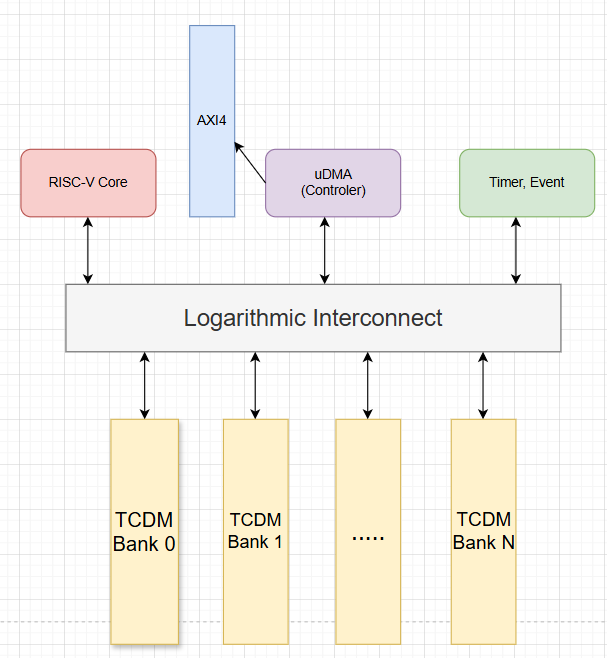
\includegraphics[width=0.8\textwidth]{chapter04/img/pulp_arch.png}  
    \caption{Sơ đồ kiến trúc nội bộ của Phân hệ PULP trên FPGA.}
    \label{fig:pulp_arch}
\end{figure}

\subsection{Cấu hình Nhân Vi xử lý (RISC-V Core Configuration)}
Trung tâm điều khiển của PL là lõi IP RISC-V (dựa trên nhân CV32E40P). Lõi này được tham số hóa trước khi tổng hợp (Synthesis) để đạt sự cân bằng tối ưu giữa tài nguyên FPGA (LUTs) và hiệu năng tính toán:

\begin{table}[h]
\centering
\caption{Thông số cấu hình RISC-V Soft-core}
\label{tab:riscv_config}
\begin{tabular}{|l|l|p{6cm}|}
\hline
\textbf{Tham số} & \textbf{Giá trị} & \textbf{Ý nghĩa thiết kế} \\ \hline
Architecture & RV32IMCXpulp & Hỗ trợ tập lệnh nhân (M), nén (C) và mở rộng DSP/SIMD (Xpulp) cho AI. \\ \hline
Pipeline Stages & 4 & Đủ sâu để đạt tần số 100MHz, đủ ngắn để giảm độ trễ rẽ nhánh. \\ \hline
FPU & Disabled & Không sử dụng bộ xử lý dấu phẩy động để tiết kiệm diện tích (MobileNet đã được lượng tử hóa sang INT8). \\ \hline
Instruction Cache & 4 KB & Kiểu Direct Mapped, giúp CPU nạp lệnh nhanh mà không cần truy cập RAM ngoài liên tục. \\ \hline
Boot Address & \texttt{0x1A00\_0000} & Vị trí vector ngắt khởi động, trỏ tới vùng nhớ ROM khởi tạo. \\ \hline
\end{tabular}
\end{table}

\subsection{Hệ thống Bộ nhớ TCDM và Interconnect}
Điểm yếu chí tử của các hệ thống đa vi xử lý là hiện tượng tranh chấp bộ nhớ (Memory Contention). Thiết kế này giải quyết triệt để vấn đề trên bằng kiến trúc TCDM (Tightly Coupled Data Memory).

\subsubsection{Tổ chức Bộ nhớ Đan xen (Interleaved Memory Banking)}
Thay vì sử dụng một khối Block RAM khổng lồ đơn nhất (64KB), bộ nhớ TCDM được chia nhỏ thành \textbf{16 ngân hàng (Banks)}, mỗi ngân hàng có dung lượng 4KB.
\begin{itemize}
    \item \textbf{Nguyên lý:} Các địa chỉ liên tiếp nhau ($Addr, Addr+4, Addr+8...$) được lưu trữ lần lượt trên các Bank khác nhau ($Bank_0, Bank_1, Bank_2...$).
    \item \textbf{Lợi ích:} Cho phép truy cập song song. Ví dụ: RISC-V Core có thể đọc dữ liệu tại địa chỉ $A$ (nằm ở Bank 0) cùng lúc uDMA ghi dữ liệu vào địa chỉ $B$ (nằm ở Bank 1) mà không hề xảy ra xung đột.
\end{itemize}

\subsubsection{Logarithmic Interconnect}
Kết nối giữa các Master (Core, uDMA) và các Slave (Memory Banks) không phải là một Bus tuyến tính mà là một \textbf{Ma trận chuyển mạch (Switch Matrix)}.
\begin{itemize}
    \item Mạng lưới này có độ trễ cực thấp (chỉ 1 chu kỳ xung nhịp).
    \item Đảm bảo băng thông cực đại: Tổng băng thông nội bộ có thể đạt tới $N \times 32$-bit/cycle (với N là số lượng Bank).
\end{itemize}

\subsection{Cơ chế Truy cập Bộ nhớ Trực tiếp (uDMA)}
Để giải phóng CPU khỏi tác vụ sao chép dữ liệu nhàm chán, một bộ điều khiển uDMA (Micro-DMA) chuyên dụng được tích hợp:
\begin{itemize}
    \item \textbf{Chức năng:} uDMA đóng vai trò cầu nối giữa các ngoại vi tốc độ cao (như AXI4 port nối tới DDR4, SPI, Camera) và bộ nhớ TCDM.
    \item \textbf{Double Buffering:} uDMA hỗ trợ cấu hình hai vùng đệm (Buffer A và Buffer B). Khi đang xử lý dữ liệu ở Buffer A, uDMA sẽ tự động tải dữ liệu mới vào Buffer B trong nền (Background).
    \item \textbf{Kết nối với Accelerator:} uDMA cung cấp một luồng dữ liệu liên tục (Stream) cho khối tăng tốc CNN thông qua giao diện AXI-Stream, đảm bảo bộ tăng tốc luôn có dữ liệu để tính toán (tránh hiện tượng Starvation).
\end{itemize}

%=============================================================
\newpage
\section{Thiết kế Khối Tăng tốc phần cứng (CNN Accelerator)}
Nằm trong PL, khối tăng tốc CNN được thiết kế để thực hiện các phép toán tích chập
một cách song song và hiệu quả. Thiết kế này bao gồm các thành phần chính \cite{fpga2}
\label{sec:cnn_accelerator}

Đây là thành phần cốt lõi quyết định hiệu năng của toàn bộ hệ thống Edge-AI. 
Để đáp ứng yêu cầu tính toán thời gian thực của mạng MobileNetV1, nhóm thực hiện thiết kế một bộ tăng tốc phần cứng chuyên dụng (Domain-Specific Architecture - DSA) được tích hợp trong miền Logic khả trình (PL).
Khối tăng tốc này được thiết kế để giảm tải (offload) các phép toán tích 
chập nặng nề nhất khỏi vi xử lý RISC-V, hoạt động theo cơ chế dòng dữ liệu 
(Dataflow) để tối đa hóa thông lượng.

\subsection{Kiến trúc tổng quát khối Accelerator}
Sơ đồ khối chức năng của bộ tăng tốc được mô tả trong Hình \ref{fig:accel_arch}. Khối này giao tiếp với hệ thống thông qua hai giao diện chính:

\begin{figure}[h]
\centering
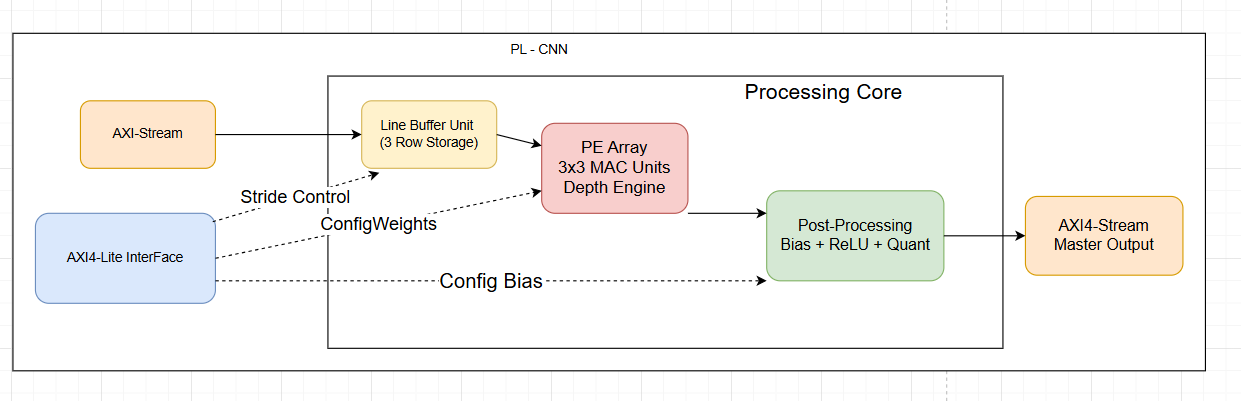
\includegraphics[width=1\textwidth]{chapter04/img/cnn_acce.png}
\caption{Sơ đồ khối chức năng chi tiết của bộ tăng tốc CNN (Accelerator Core Architecture).}
\label{fig:accel_arch}
\end{figure}

\begin{itemize}
    \item \textbf{AXI4-Stream Slave:} Nhận dòng pixel ảnh đầu vào từ uDMA hoặc trực tiếp từ bộ nhớ đệm.
    \item \textbf{AXI4-Stream Master:} Đẩy dòng kết quả (Feature Maps) sau khi tính toán trở lại bộ nhớ.
\end{itemize}

\subsection{Các thành phần chức năng chi tiết}

\subsubsection{Bộ đệm dòng (Line Buffer)}
Để thực hiện tích chập $3 \times 3$, tại mỗi thời điểm cần truy cập đồng thời 3 hàng pixel liên tiếp. Nếu đọc trực tiếp từ DDR cho mỗi lần trượt cửa sổ thì băng thông sẽ trở thành điểm nghẽn. Thiết kế sử dụng \textit{line buffer} hai-bank dựa trên BRAM nội bộ với cơ chế \textit{read-before-write parity-toggled}: khi một pixel mới được nạp vào bank này thì 2 hàng cũ vẫn được giữ ở bank kia. Cùng với khối \texttt{window\_3x3} đứng sau (mảng thanh ghi $3 \times 3 \times \texttt{cin}$), thiết kế tái sử dụng dữ liệu cục bộ và giảm số lần truy xuất bộ nhớ ngoài xuống còn 1 lần/pixel.

\subsubsection{Mảng tính toán PE và adder tree}
Trung tâm tính toán của bộ tăng tốc gồm 9 PE (Processing Element) MAC (Multiply-Accumulate) hoạt động song song, tương ứng với 9 vị trí của kernel $3 \times 3$:
\begin{itemize}
    \item Mỗi PE thực hiện phép nhân INT8$\times$INT8 và cộng dồn vào thanh ghi tích lũy 32-bit. Cấu trúc pipelined với MREG + PREG cho phép Vivado ánh xạ trực tiếp vào khối DSP48E2.
    \item Đầu ra của 9 PE được tổng hợp qua \textit{adder tree} 4-tầng để cho ra một giá trị tích chập 32-bit cho mỗi nhóm 9 pixel + 9 trọng số.
    \item Đối với layer có nhiều kênh đầu vào ($\texttt{cin} > 1$), bộ điều khiển sử dụng cơ chế \textit{channel-interleaved per pixel}: tích lũy qua \texttt{cin} kênh trước khi xuất ra giá trị OFM cho mỗi tổ hợp $(y, x, \texttt{cnt\_cout})$.
\end{itemize}

\subsubsection{Khối lượng tử hóa (Requantize)}
Sau khi tổng chập, kết quả 32-bit cần được \textit{re-quantize} về INT8 để khớp định dạng đầu vào của layer kế tiếp. Khối \texttt{requantize.sv} thực hiện đường ống 3-tầng theo công thức TFLite \cite{jacob2018quantization}:
\begin{equation}
    y_q = \mathrm{sat}_{\mathrm{INT8}}\!\left( \left\lfloor \frac{(\sum x \cdot w + b) \cdot M_{q31} + 2^{30+n}}{2^{31+n}} \right\rfloor + z_{\mathrm{out}} \right)
\end{equation}
trong đó $M_{q31}$ là hệ số nhân Q31 (\texttt{int32}), $n$ là số bit dịch phải ($n \in [0, 31]$), $z_{\mathrm{out}}$ là zero-point đầu ra. Cờ \texttt{has\_relu} điều khiển việc kẹp giá trị âm về 0 (fused ReLU). Hệ số $M_{q31}$ và $n$ được tính sẵn trong pipeline huấn luyện và truyền xuống qua thanh ghi S00\_AXI cho từng layer.

\subsection{Đặc tính thiết kế và tối ưu cho vgg-tiny}
\label{sec:accel_optimize}
Thay vì cố gắng tổng quát hóa hỗ trợ tất cả các loại mạng CNN, đề tài chọn \textbf{thu hẹp tập op} mà bộ tăng tốc hỗ trợ trong phiên bản v2.0 alpha để đảm bảo tiến độ và tính đúng đắn:
\begin{itemize}
    \item Hỗ trợ Conv 3$\times$3 với padding VALID, stride 1, hàm kích hoạt ReLU (fused).
    \item Hỗ trợ tới \texttt{MAX\_CIN} = 64 và \texttt{MAX\_COUT} = 64 kênh trên mỗi layer (tham số hóa trong \texttt{conv\_pkg.sv}).
    \item Hỗ trợ runtime-configurable cho geometry ($W \times H$), số kênh, hệ số lượng tử hóa qua thanh ghi điều khiển AXI4-Lite.
\end{itemize}

Lựa chọn này dẫn đến mô hình triển khai chính là \texttt{vgg-tiny} -- một mạng \textit{fully-convolutional} đơn giản chỉ dùng các op nói trên (mục~\ref{sec:vgg_tiny}). Các kiến trúc phức tạp hơn như Pointwise 1$\times$1, Depthwise, Stride 2, Padding SAME, hay Residual Add được dành cho các pha mở rộng tương lai trong roadmap (mục~\ref{sec:tier_roadmap}).

%=============================================================
%
%=============================================================
\newpage
\section{Mô hình AI mục tiêu: vgg-tiny}
\label{sec:ai_algorithm}

Việc lựa chọn mô hình AI chạy trên hệ thống phải cân bằng giữa hai yếu tố: (i) tập op mà bộ tăng tốc Conv-CNN v2.0 hỗ trợ (xem mục~\ref{sec:accel_optimize}) và (ii) độ chính xác đủ tốt cho bài toán phân loại nhị phân. Đề tài đề xuất một kiến trúc tinh gọn riêng tên \texttt{vgg-tiny} -- lấy cảm hứng từ phong cách VGG (chỉ dùng Conv $3 \times 3$ stacking) nhưng được rút gọn để chạy được hoàn toàn trên phần cứng đã thiết kế.

\subsection{Đặc tả kiến trúc vgg-tiny}
\label{sec:vgg_tiny}
\texttt{vgg-tiny} là một mạng \textit{fully-convolutional} 5 layer, đầu vào ảnh RGB $128 \times 128$, output là tensor 2 kênh được ARM thực hiện Global Average Pooling + softmax + argmax thành nhãn cuối cùng. Bảng~\ref{tab:vgg_tiny_layers} mô tả cấu trúc chi tiết.

\begin{table}[h]
\centering
\caption{Cấu trúc chi tiết các lớp mạng vgg-tiny (đầu vào $128 \times 128 \times 3$, lượng tử hóa INT8)}
\label{tab:vgg_tiny_layers}
\begin{tabular}{|c|l|c|c|c|c|}
\hline
\textbf{Layer} & \textbf{Loại op} & \textbf{IFM} & \textbf{OFM} & \textbf{Kernel} & \textbf{Activation} \\ \hline
L0 & Conv2D + ReLU & $128 \times 128 \times 3$ & $126 \times 126 \times 8$ & $3 \times 3$ & ReLU \\ \hline
L1 & Conv2D + ReLU & $126 \times 126 \times 8$ & $124 \times 124 \times 16$ & $3 \times 3$ & ReLU \\ \hline
L2 & Conv2D + ReLU & $124 \times 124 \times 16$ & $122 \times 122 \times 32$ & $3 \times 3$ & ReLU \\ \hline
L3 & Conv2D + ReLU & $122 \times 122 \times 32$ & $120 \times 120 \times 64$ & $3 \times 3$ & ReLU \\ \hline
L4 & Conv2D (logits) & $120 \times 120 \times 64$ & $118 \times 118 \times N$ & $3 \times 3$ & None \\ \hline
\multicolumn{6}{|l|}{\textit{Hậu xử lý trên ARM:} GAP $\to$ softmax $\to$ argmax $\to$ nhãn ($N = $ số lớp = 2)} \\ \hline
\end{tabular}
\end{table}

Các đặc điểm chính:
\begin{itemize}
    \item \textbf{Tất cả op đều thuộc tập hỗ trợ của bộ tăng tốc:} Conv $3 \times 3$, padding VALID, stride 1, ReLU fused. Layer cuối cùng (\texttt{L4}) tắt activation để xuất logits cho softmax trên ARM.
    \item \textbf{Không có Dense head:} Layer cuối là Conv $3 \times 3$ với $\texttt{cout} = N$ (số lớp), thay vì Conv $\to$ Flatten $\to$ Dense kiểu VGG truyền thống. Cách này loại bỏ nhu cầu phần cứng hỗ trợ Fully Connected layer.
    \item \textbf{Không có MaxPool} trong v2.0 alpha: kích thước feature map giảm dần qua valid-padding ($-2$ pixel mỗi chiều). Kết quả là feature map cuối tương đối lớn ($118 \times 118$) và latency cao hơn so với phiên bản có pool. Việc bổ sung MaxPool 2$\times$2 hoặc Conv stride-2 được dành cho V2.1.
    \item \textbf{Số tham số nhỏ:} Tổng cộng $\approx 25,700$ tham số INT8 (xem chi tiết tại bảng~\ref{tab:vgg_tiny_perlayer} trong chương~\ref{chp:06}), dung lượng weights blob khoảng 25 KB -- nằm gọn trong bộ nhớ DDR và dễ quản lý.
\end{itemize}

\subsection{So sánh vgg-tiny với các mô hình thông dụng}
Để minh chứng cho lựa chọn thiết kế, bảng~\ref{tab:model_comparison} so sánh \texttt{vgg-tiny} với các kiến trúc CNN phổ biến trên cùng tiêu chí:

\begin{table}[h]
\centering
\caption{So sánh vgg-tiny với các mạng CNN phổ biến}
\label{tab:model_comparison}
\resizebox{\textwidth}{!}{%
\begin{tabular}{|l|c|c|r|r|r|c|}
\hline
\textbf{Mô hình} & \textbf{Input} & \textbf{Số layer} & \textbf{Params} & \textbf{INT8 size} & \textbf{MACs} & \textbf{FPGA-deployable} \\ \hline
\texttt{vgg-tiny} & $128 \times 128$ & 5 & 25.7K & 25.1 KB & 371 M & \cmark \\ \hline
VGG11 / VGG16 & $224 \times 224$ & 13 & 14.7M & 14.4 MB & 15{,}347 M & \xmark{} (FC head + pool stride-2) \\ \hline
ResNet-18 (V2) & $224 \times 224$ & 53 & 23.6M & 23.0 MB & 3{,}480 M & \xmark{} (1$\times$1 + BN + residual) \\ \hline
EfficientNet-B0 & $224 \times 224$ & 81 & 4.05M & 3.96 MB & 385 M & \xmark{} (depthwise + SE + swish) \\ \hline
MobileNetV1/V2 & $224 \times 224$ & 28 & 2.3--4.2M & 2.2--4.0 MB & 300--569 M & \xmark{} (depthwise) \\ \hline
\end{tabular}%
}
\end{table}

So với các mô hình thương mại, \texttt{vgg-tiny} nhỏ gọn hơn từ 100$\times$ đến 900$\times$ về số tham số, đồng thời tránh được hoàn toàn các op khó (depthwise, BN, residual, SE). Đánh đổi là không gian biểu diễn (representation capacity) hạn chế, phù hợp với bài toán phân loại nhị phân nhưng chưa đủ cho bài toán phân loại nhiều lớp phức tạp như ImageNet 1000 classes.

\subsection{Lộ trình mở rộng (Tier Roadmap)}
\label{sec:tier_roadmap}
Đề tài định hướng triển khai mở rộng theo ba tier, với \texttt{vgg-tiny} là Tier 1 (đã xong), Tier 2--3 là các pha mở rộng:

\begin{itemize}
    \item \textbf{Tier 1 -- vgg-tiny (đã triển khai):} Chỉ Conv $3 \times 3$ stride-1 valid + ReLU. Bộ tăng tốc v2.0 alpha.
    \item \textbf{Tier 2 -- VGG11 / ResNet-18 (mở rộng):} Bổ sung MaxPool 2$\times$2 (hoặc stride-2 conv), padding SAME, 1$\times$1 conv, residual addition. Yêu cầu mở rộng \texttt{conv\_core.sv} và \texttt{controller\_fsm.sv} nhưng không thay đổi giao thức AXI hay layer table contract.
    \item \textbf{Tier 3 -- ResNet-50 / YOLOv3-Tiny (stretch):} Thêm BN folding offline, leaky-ReLU, upsample $2\times$ cho detection head.
\end{itemize}

Mọi mở rộng đều \textbf{không phá vỡ ABI v2.0}: chỉ cần thêm enum cho \texttt{activation\_t}/\texttt{padding\_t}/\texttt{kernel\_size} trong \texttt{layer\_desc.h} và thêm 1 mode-bit ở conv\_core MUX. Pipeline huấn luyện và phần mềm host không cần thay đổi.

\subsection{Lượng tử hóa (Quantization)}
Vi xử lý RISC-V và Khối tăng tốc phần cứng trên FPGA được thiết kế để xử lý số nguyên (Integer Arithmetic) nhằm tối đa hóa tốc độ và tiết kiệm bộ nhớ. Do đó, mô hình gốc (Float32) cần trải qua quy trình \textit{Post-training Quantization}:

\begin{itemize}
    \item \textbf{Weights (Trọng số):} Chuyển đổi từ \texttt{float32} (4 bytes) sang \texttt{int8} (1 byte).
    \item \textbf{Activations (Giá trị kích hoạt):} Đầu ra của mỗi lớp cũng được ép về \texttt{int8}.
    \item \textbf{Bias (Hệ số chệch):} Lưu trữ dưới dạng \texttt{int32} để tránh tràn số (overflow) khi cộng dồn, sau đó được dịch bit (bit-shift) để quay về \texttt{int8}.
\end{itemize}

Công thức lượng tử hóa tổng quát được áp dụng:
\begin{equation}
    R = S(Q - Z)
\end{equation}
Trong đó $R$ là giá trị thực (Real value), $Q$ là giá trị lượng tử hóa (Quantized value), $S$ là tỷ lệ (Scale) và $Z$ là điểm không (Zero-point).

\subsection{Tổ chức Dữ liệu trong Bộ nhớ}
Để tối ưu hóa cho việc truy cập Burst qua AXI4 Bus (128-bit width), các ma trận trọng số (Weights) không được lưu trữ theo thứ tự tuyến tính thông thường mà được sắp xếp lại (Memory Packing):
\begin{itemize}
    \item \textbf{Kernel Layout:} Các bộ lọc được sắp xếp theo cấu trúc \texttt{OHWI} 
    (Output-Height-Width-Input) để đảm bảo khi uDMA đọc 16 bytes (128-bit) sẽ thu được 
    đủ dữ liệu cho các bộ nhân hoạt động song song.
    \item \textbf{C-Header Generation:} File mô hình \texttt{.tflite} cuối cùng được
     chuyển đổi (dump) thành các mảng hằng số trong ngôn ngữ C (\texttt{weights.h})
      để biên dịch cùng với Firmware của RISC-V.
\end{itemize}

%=============================================================
\section{Luồng thực thi và Giao thức bắt tay}
\label{sec:system_flow}

Trong kiến trúc dị thể, việc đồng bộ hóa giữa vi xử lý ARM (chạy Linux + PYNQ runtime) và lõi RISC-V (chạy bare-metal) là yếu tố quyết định tính đúng đắn của hệ thống. Đề tài sử dụng cơ chế bắt tay dựa trên các thanh ghi trạng thái trong D-BRAM Port B (đã trình bày tại mục~\ref{sec:handshake_regs}). Phần này mô tả luồng thực thi end-to-end cho một lần inference.

\paragraph{Quy trình inference một ảnh}
Quá trình thực thi diễn ra qua 4 pha tuần tự, được minh họa trong sơ đồ tuần tự Hình~\ref{fig:sequence_diagram}:

\begin{enumerate}
    \item \textbf{Pha 1 -- ARM chuẩn bị dữ liệu:}
    \begin{itemize}
        \item ARM đọc ảnh \texttt{.jpg}/\texttt{.png} từ thẻ nhớ SD bằng \texttt{cv2.imread}.
        \item Tiền xử lý: chuyển BGR$\to$RGB, resize về $128 \times 128$, chuẩn hóa $[0,1]$.
        \item Lượng tử hóa INT8 theo công thức $q = \mathrm{round}(x / S_{\mathrm{in}}) + Z_{\mathrm{in}}$ với $S_{\mathrm{in}}, Z_{\mathrm{in}}$ đọc từ \texttt{meta.json}.
        \item Cấp phát ba CMA buffer qua \texttt{pynq.allocate}: \texttt{wbuf} (weights), \texttt{buf\_a} (IFM ping-pong), \texttt{buf\_b} (scratch ping-pong); ghi pixel ảnh đã lượng tử vào \texttt{buf\_a} và gọi \texttt{flush()}.
        \item Ghi 3 thanh ghi địa chỉ vật lý \texttt{IFM\_PHYS\_ADDR}, \texttt{OFM\_PHYS\_ADDR}, \texttt{WEIGHT\_BASE} và \texttt{DATASET\_ID} vào D-BRAM Port B (mục~\ref{sec:handshake_regs}).
    \end{itemize}

    \item \textbf{Pha 2 -- ARM kích hoạt RISC-V:}
    \begin{itemize}
        \item Ghi \texttt{0x01} (START) vào \texttt{CMD\_FROM\_ARM @ 0xB004\_0000}.
        \item ARM chuyển sang chế độ chờ (polling \texttt{STATUS\_TO\_ARM} hoặc đợi IRQ).
    \end{itemize}

    \item \textbf{Pha 3 -- RISC-V điều phối tính toán:}
    \begin{itemize}
        \item RISC-V phát hiện \texttt{CMD\_FROM\_ARM == 0x01}, ghi \texttt{STATUS\_TO\_ARM = 0x01} (BUSY).
        \item Duyệt mảng \texttt{LAYERS[]} (compile-in trong I-BRAM): với mỗi layer $i$:
        \begin{itemize}
            \item Tính địa chỉ vật lý weight = \texttt{WEIGHT\_BASE + LAYERS[i].weight\_offset}; ping-pong: \texttt{in = (i\&1)?buf\_b:buf\_a}, \texttt{out = ngược lại}.
            \item Cấu hình \texttt{conv\_cnn\_0/S00\_AXI}: ghi geometry, channels, $M_{q31}$, shift, zero-point, có ReLU; chuyển sang chế độ load weight.
            \item Lập trình \texttt{axi\_dma\_0}: MM2S đọc weights từ DDR $\to$ \texttt{conv\_cnn\_0/S00\_AXIS}; chờ done.
            \item Chuyển sang chế độ infer; lập trình DMA tiếp: MM2S đọc IFM, S2MM ghi OFM về DDR; chờ done.
        \end{itemize}
        \item Sau layer cuối, ghi \texttt{STATUS\_TO\_ARM = 0x02} (DONE).
    \end{itemize}

    \item \textbf{Pha 4 -- ARM hậu xử lý:}
    \begin{itemize}
        \item ARM phát hiện \texttt{STATUS\_TO\_ARM == 0x02}, gọi \texttt{.invalidate()} trên buffer chứa OFM cuối (xác định bởi \texttt{final\_ofm\_buf\_idx} trong \texttt{meta.json}).
        \item Thực hiện Global Average Pool trên trục $(H, W)$ của tensor INT8 OFM, sau đó dequantize về float, áp dụng softmax, lấy argmax để có nhãn cuối cùng.
        \item Hiển thị kết quả lên notebook (matplotlib overlay), in ra console hoặc lưu file log.
        \item Ghi \texttt{CMD\_FROM\_ARM = 0x00} (IDLE) để sẵn sàng cho ảnh tiếp theo.
    \end{itemize}
\end{enumerate}

\begin{figure}[!h]
    \centering
    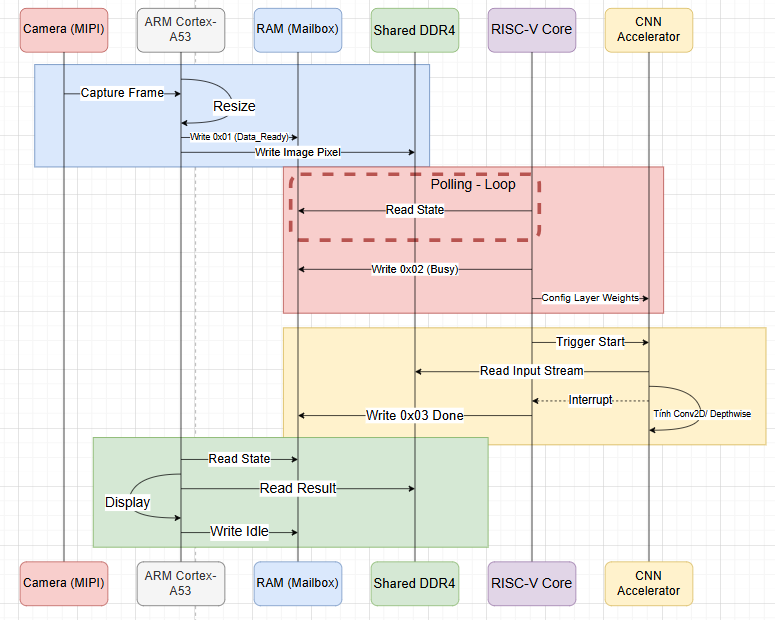
\includegraphics[width=1\textwidth]{chapter04/img/flow.png}
    \caption{Sơ đồ quy trình}
    \label{fig:sequence_diagram}
\end{figure}